\begin{figure}
  \centering
  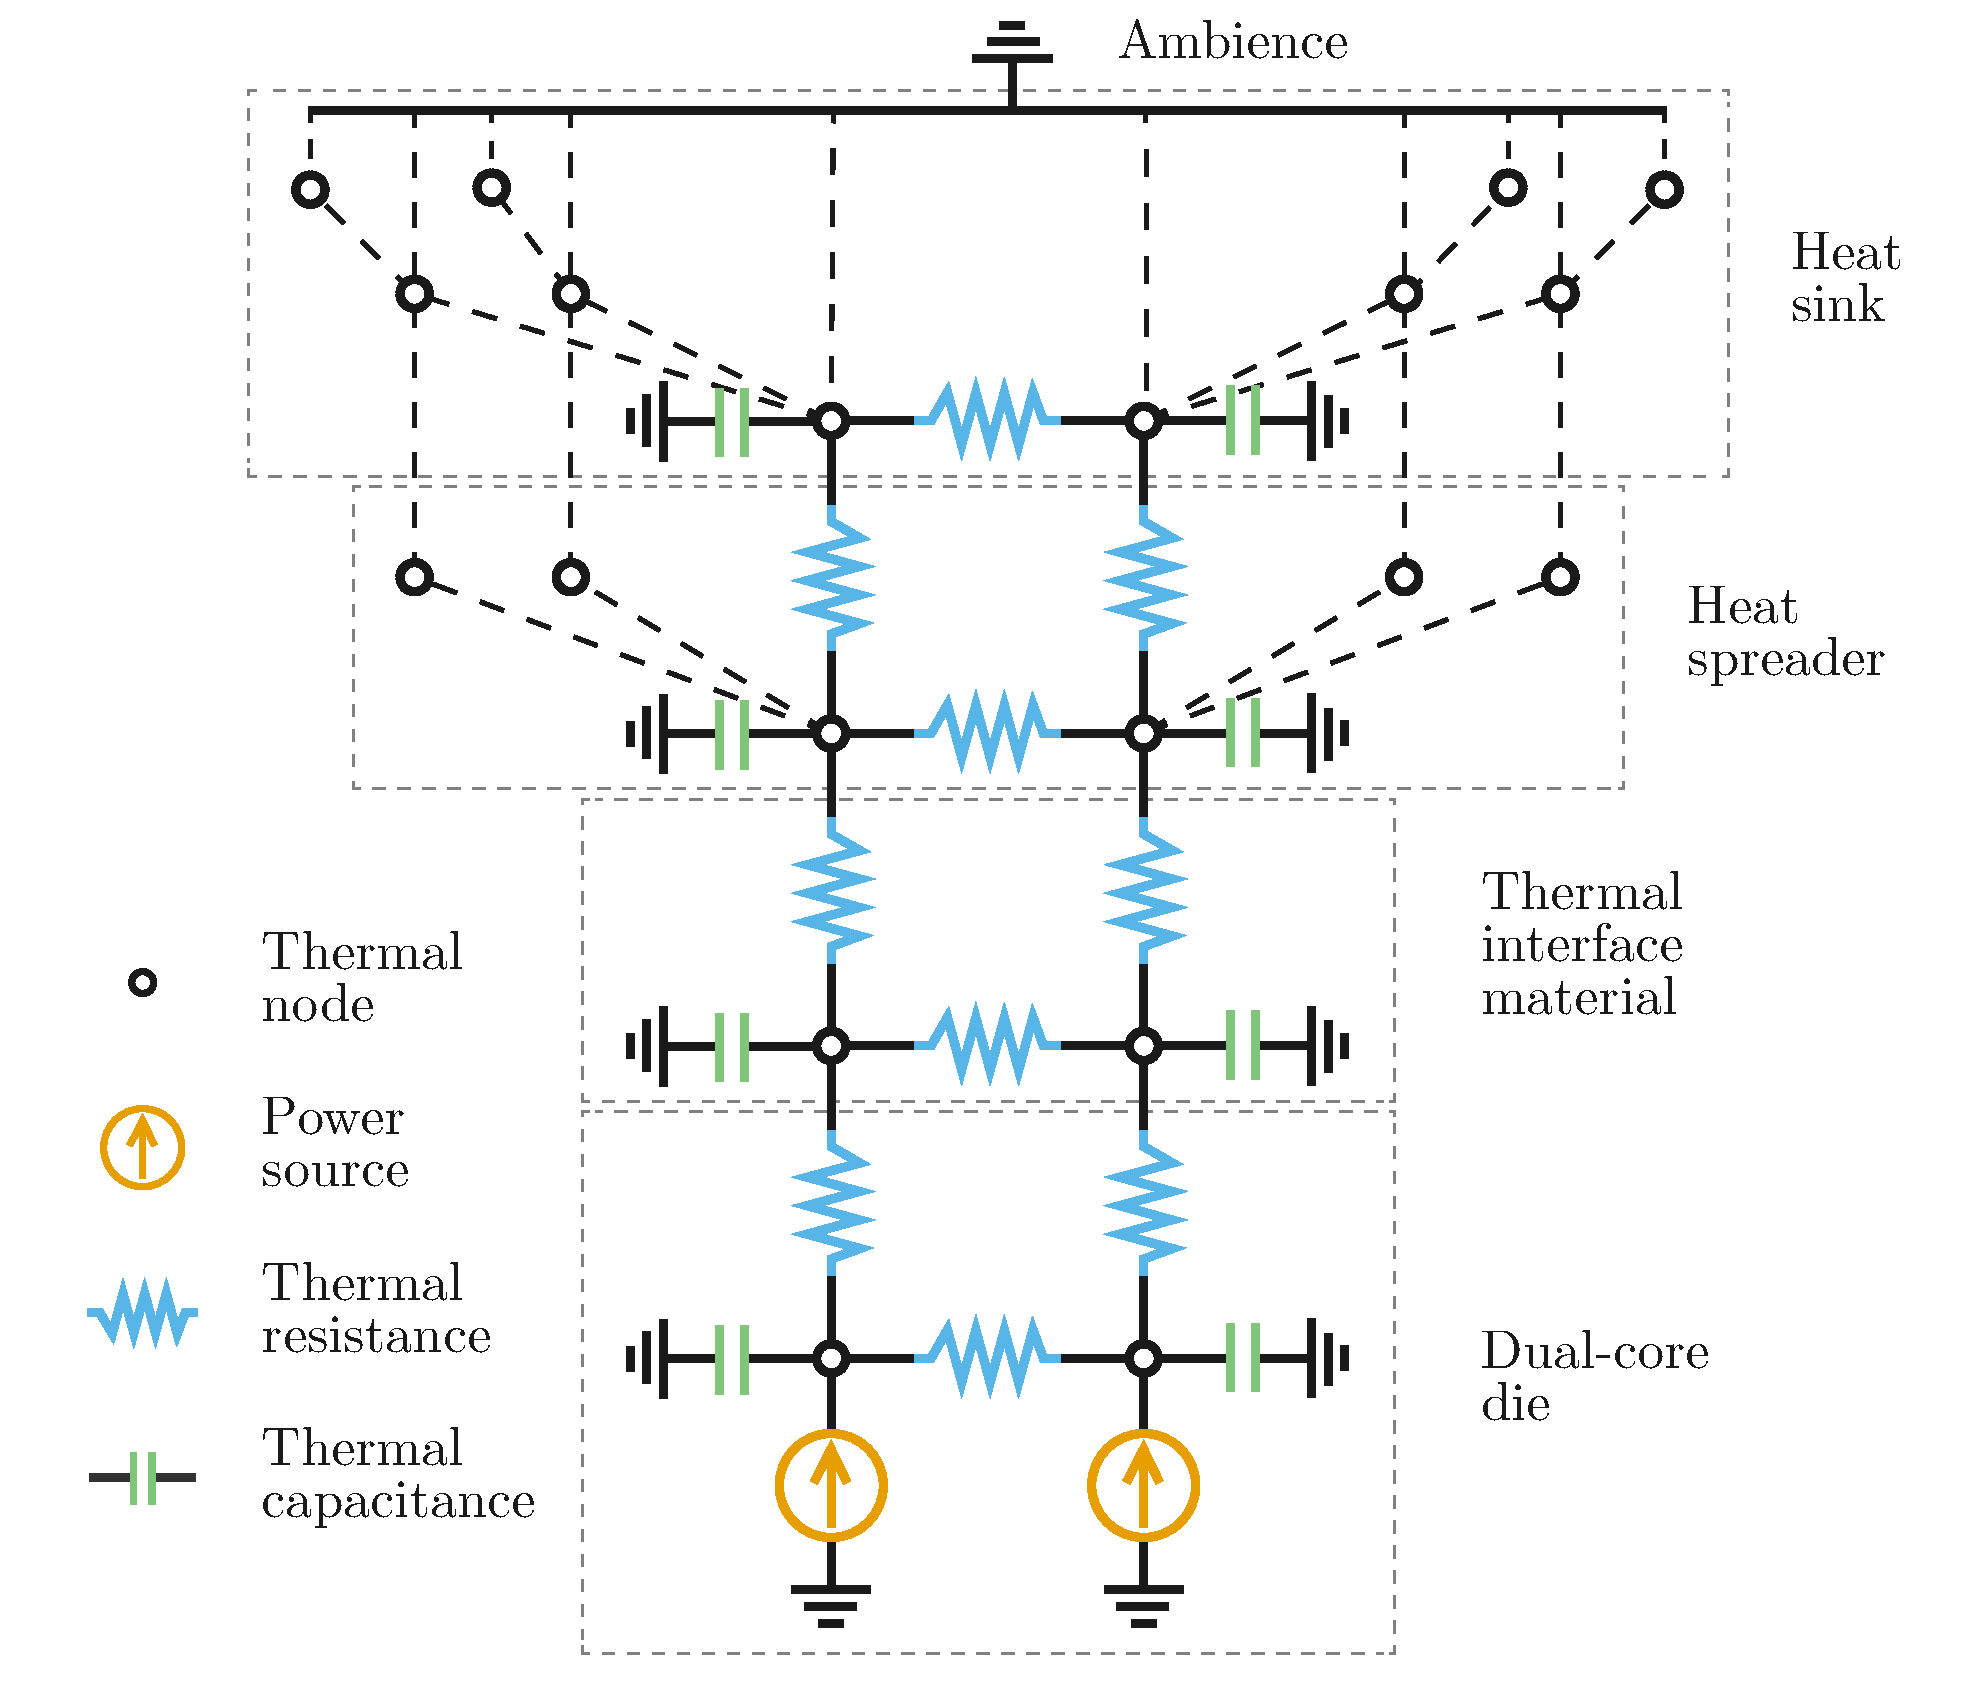
\includegraphics[width=\linewidth]{include/assets/circuit.pdf}
  \vspace{-1.0em}
  \caption{A simplified thermal RC circuit of a dual-core platform with a three-layer thermal package.}
  \flabel{circuit}
  \vspace{-1.5em}
\end{figure}

We move on to \stage{3}\ where the thermal model of the multiprocessor system is to be established.
Given the thermal specification $\system$ of the considered platform (the floorplan of the die, the configuration of the thermal package, \etc), we employ HotSpot (v5.02) \cite{hotspot} in order to construct the equivalent thermal RC circuits of the system.
Specifically, we are interested in the coefficient matrices $\mCF(\t)$ and $\mCS(\t)$ in \eref{fourier-system} (see also \fref{algorithm}), which HotSpot helps us to compute by providing the corresponding capacitance and conductance matrices of the system as described in \aref{thermal-model}.
In this case, thermal packages are modeled with three layers, and the relation between the number of processing elements and the number of thermal nodes is given by $\nnodes = 4 \nprocs + 12$.
An example of such a circuit for a dual-core platform is depicted in \fref{circuit}.

To conclude, the power and thermal models of the platform are now acquired, and we are ready to construct the corresponding surrogate model \via\ PC expansions.
